%% abtex2-modelo-trabalho-academico.tex, v<VERSION> laurocesar
%% Copyright 2012-<COPYRIGHT_YEAR> by abnTeX2 group at http://www.abntex.net.br/ 

\documentclass[
	% -- opções da classe memoir --
	12pt,				% tamanho da fonte
	oneside,			% para impressão mudar para twoside para facilitar impressaõ de frente e verso 
	a4paper,			% tamanho do papel. 
	chapter=TITLE,
	sumario=tradicional,
	% -- opções do pacote babel --
	english,			% idioma adicional para hifenização
	brazil				% o último idioma é o principal do documento
]{abntex2}

% ----------------------------------------------------------
% IMPORTAÇÃO DE PACOTES
% ----------------------------------------------------------
\usepackage{helvet}
\renewcommand{\familydefault}{\sfdefault}			% Usa a fonte Arial			
\usepackage[T1]{fontenc}		% Selecao de codigos de fonte.
\usepackage[utf8]{inputenc}		% Codificacao do documento (conversão automática dos acentos)
\usepackage{indentfirst}		% Indenta o primeiro parágrafo de cada seção.
\usepackage{color}				% Controle das cores
\usepackage{graphicx}			% Inclusão de gráficos
\usepackage{microtype} 			% para melhorias de justificação
\usepackage{hyperref}
\usepackage{times}

\usepackage{amsmath}
\usepackage{amsthm,amsfonts}

\usepackage{lipsum}				% para geração de dummy text
\usepackage{import}
\usepackage{blindtext}
\usepackage{soul}
\usepackage{lscape}

\graphicspath{ {./images/} }

% ---
% Pacotes de citações
% ---
\usepackage[alf]{abntex2cite}	% Citações padrão ABNT

% ----------------------------------------------------------
% CONFIGURAÇÕES DO PDF
% ----------------------------------------------------------

% alterando o aspecto da cor azul
\definecolor{blue}{RGB}{41,5,195}
\definecolor{black}{RGB}{0,0,0}

% informações do PDF
\makeatletter
\hypersetup{
     	%pagebackref=true,
		pdftitle={\@title}, 
		pdfauthor={\@author},
    	pdfsubject={\imprimirpreambulo},
	    pdfcreator={LaTeX with abnTeX2},
		pdfkeywords={abnt}{latex}{abntex}{abntex2}{trabalho acadêmico}, 
		colorlinks=true,       		% false: boxed links; true: colored links
    	linkcolor=black,          	% color of internal links
    	citecolor=black,        		% color of links to bibliography
    	filecolor=black,      		% color of file links
		urlcolor=black,
		bookmarksdepth=4
}
\makeatother

\setlrmarginsandblock{3cm}{2cm}{*}
\setulmarginsandblock{3cm}{2cm}{*}
\checkandfixthelayout

% --- 

% ----------------------------------------------------------
% FIGURAS E TABELAS
% ----------------------------------------------------------

% ---
% Posiciona figuras e tabelas no topo da página quando adicionadas sozinhas
% em um página em branco. Ver https://github.com/abntex/abntex2/issues/170
\makeatletter
\setlength{\@fptop}{5pt} % Set distance from top of page to first float
\makeatother
% ---

% ----------------------------------------------------------
% ESPAÇAMENTOS
% ----------------------------------------------------------

% O tamanho do parágrafo é dado por:
\setlength{\parindent}{1.25cm}

% % Controle do espaçamento entre um parágrafo e outro:
\setlength{\parskip}{0.2cm} 

\setlength{\ABNTEXcitacaorecuo}{4cm}

% Espaçamento entre headers e texto abaixo
\setlength\afterchapskip{0.2cm}
\setlength\aftersecskip{0.2cm} %espaçamento entre seção e texto
\setlength\aftersubsecskip{0.2cm} %espaçamento entre subseção e texto

% ----------------------------------------------------------
% CORREÇÕES DE ESTILO
% ----------------------------------------------------------

% Estilos das legendos
\captionnamefont{\ABNTEXfontereduzida}
\captiontitlefont{\ABNTEXfontereduzida}
\setlength{\belowcaptionskip}{1pt} % espaçamento depois do título das tabelas/figuras
\setlength{\abovecaptionskip}{1pt} % espaçamento antes da legenda de tabelas/figuras

% Estilos dos títulos

\renewcommand{\ABNTEXchapterfontsize}{\bfseries\normalsize}
\renewcommand{\ABNTEXsectionfontsize}{\itshape\normalsize}
\renewcommand{\ABNTEXsubsectionfontsize}{\normalfont\normalsize}
\renewcommand{\ABNTEXsubsubsectionfontsize}{\normalfont\normalsize}

\renewcommand{\chaptitlefont}{\normalfont\bfseries}
\setsecheadstyle{\normalfont\itshape}
\setsubsecheadstyle{\normalfont}
\setsubsubsecheadstyle{\normalfont}

\renewcommand{\ABNTEXchapterfont}{\bfseries}
\renewcommand{\ABNTEXchapterfontsize}{\normalsize}
\setboolean{ABNTEXupperchapter}{true}

% Estilos nos sumários
\renewcommand{\cftchapterfont}{\MakeUppercase}
\setboolean{ABNTEXupperchapter}{true}

\renewcommand{\cftsectionfont}{\normalfont}
\renewcommand{\cftsubsectionfont}{\normalfont}
\renewcommand{\cftsubsubsectionfont}{\normalfont}

% ----------------------------------------------------------
% COMPILA O ÍNDICE
% ----------------------------------------------------------
\makeindex

% ----------------------------------------------------------
% COMANDOS CUSTOMIZADOS
% ----------------------------------------------------------
\newcommand{\un}[1]{\;\text{#1}}
\newcommand{\logo}{\quad \Rightarrow \quad}
\newcommand{\codeword}[1]{\texttt{\textcolor{black}{#1}}}
\newcommand{\specialcell}[2][c]{%
  \begin{tabular}[#1]{@{}c@{}}#2\end{tabular}}

% ----------------------------------------------------------
% INÍCIO DO DOCUMENTO
% ----------------------------------------------------------
\begin{document}

%\selectlanguage{english}
\selectlanguage{brazil}

% Retira espaço extra obsoleto entre as frases.
\frenchspacing 

% ----------------------------------------------------------
% ELEMENTOS PRÉ-TEXTUAIS
% ----------------------------------------------------------
\begin{center}
\textbf{UNIVERSIDADE FEDERAL DE MINAS GERAIS\\
Escola de Engenharia \\
Curso de Bacharelado em Engenharia de Sistemas}

\vspace{4cm}

%\hspace{0.3\textwidth} \parbox{0.65\textwidth}
Cleyton Luan Nobre Assis 2021019815 \\
Maria Clara Oliveira Domingos Ruas 2021019572 \\
Raphael Henrique Braga Leivas 2020028101

\vspace{4cm}  

{ \textbf{Laboratório de Circuitos Eletrônicos e Projetos - Prática 2} }

\vfill
%\hspace{0.3\textwidth} 
{Belo Horizonte \\
2025 }
\end{center}

\newpage

% ---
% inserir o sumario
% ---
\pdfbookmark[0]{\contentsname}{toc}
\tableofcontents*
\cleardoublepage
% ---

% % ----------------------------------------------------------
% % ELEMENTOS TEXTUAIS
% % ----------------------------------------------------------
\textual

\pagestyle{simple}
	
\chapter{Objetivos}\label{cap:objetivos} 

\lipsum[1-2]

\chapter{Introdução}\label{cap:introdução} 

A \autoref{fig:exemplo} é um exemplo de figura referenciável.

\begin{figure}[h!]
	\caption{\label{fig:exemplo}Panda EXEMPLO}
	\begin{center}
    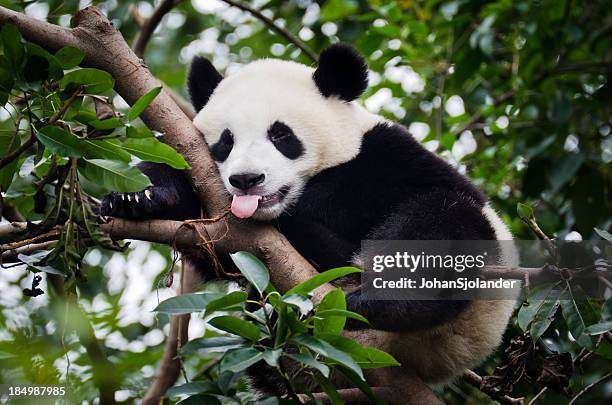
\includegraphics[width=0.8\textwidth,trim=1 1 1 1,clip]{images/random-panda.jpg}
	\end{center}
	\legend{Fonte: elaboração própria.}
\end{figure}

A \autoref{tab:minhaTabela} é um exemplo de tabela referenciável. 

\begin{table}[htb]
	\caption{Exemplo TABELA.}
	\centering
	\begin{tabular}{c|l|l}
		\textbf{Tipo} & \textbf{Interface} & \textbf{Implementação}\\ \hline
		Entradas & 
			\begin{tabular}{l} 
				Potência do Drone \\ 
				Comando do Drone \\
				Regulagem Alta Tensão \\
				Regulagem Taxa de Fluxo
			\end{tabular} & 
			\begin{tabular}{l} 
				Conector JST-XH de 2 pinos J7 \\ 
				Conector JST-XH de 2 pinos J9 \\
				Potenciômetro em J2 \\
				Potenciômetro em J8
			\end{tabular}     \\ \hline
		Saídas & 
			\begin{tabular}{l} 
				Status \\ 
				Alta Tensão \\
				Líquido
			\end{tabular} & 
			\begin{tabular}{l} 
				Conector JST-XH de 2 pinos J9 \\ 
				Conectores banana J3 e J1 \\
				Seringa da bomba projetada
			\end{tabular}     \\ 
	\end{tabular}
	\label{tab:minhaTabela}
	\legend{Fonte: elaboração própria.}
\end{table}

\lipsum[1-2]

\chapter{Desenvolvimento}

\section{Experimento 1}

\subsection{Descrição}

\subsection{Resultados Obtidos}

\subsection{Discussão}

\lipsum[1-2]

\chapter{Conclusão}\label{cap:conclusao} 

\lipsum[1-2]


\chapter{Referências}\label{cap:referencias} 

\lipsum[1-2]


\end{document}
